%# -*- coding: utf-8-unix -*-
%%==================================================
%% chapter02.tex for SJTU Master Thesis
%% based on CASthesis
%% modified by wei.jianwen@gmail.com
%% Encoding: UTF-8
%%==================================================


\chapter{基于规范的入侵检测设计}
\label{chap:spec detection}

\section{引言}
\label{sec:intro}
在上一章节中我们讨论了如何对控制器与物理设备交互的输入输出信号进行检测保护,防御对象系统主要是故障和异常数据注入攻击,为此我们还专门设计错误序列注入攻击对其进行仿真验证。但是对控制器本身尤其是PLC这种可编程控制器,由于它们在整个控制系统中发挥至关重要的作用,近年来正成为对物理设备损坏性攻击的有吸引力的目标。最为典型的Stuxnet病毒可以向PLC上传恶意代码,以物理损坏他们控制的离心机。更有研究发现,PLC控制器不仅容易被端口扫描,而且还可以被修改控制系统特定协议和被访问诊断系统。这些易受攻击的互联网控制器被计算机搜索引擎暴露,例如Shodan。所以对可编程控制器本身控制程序和指令的保护并使其免受恶意代码注入的保护也同样重要。本章我们提出了基于规范的的入侵检测来应对控制器的恶意代码注入攻击,只有经过验证合法的程序和指令才能操作系统或控制服务器上传到指定的可编程控制器设备中。

\section{入侵检测方案概述}
\label{sec:list}

本文我们采用PLC作为待检测可编程控制器,检测机制作为外部单独的功能处理器BITS(Bump-in-the-wire)模式放置在控制系统网络和PLC之间。对于任何等待上传到工业设备的PLC代码,将被拦截并验证由过程安全工程师定义的一整套安全规范(safety properties),安全特性的示例包括数字设备参数(例如最大驱动速度和加速度)和安全互锁的界限并确保不发生物理上冲突的事件。图\ref{fig21}展示了基于规范入侵检测机制的基本过程,首先将PLC代码(IL code)格式化整理并通过IL2boolIL算法转换为中间语言,我们定义为布尔逻辑指令表代码(Boolean IL code),旨在使抽象程序逻辑清晰更具一般性。然后布尔逻辑指令表代码通过模板实例化(Template Instantiate
)过程被迭代地执行将通用模板代码实例化为验证工具NuSMV输入程序。前面两步是对PLC程序的形式化建模过程,接下来我们给出验证过程。我们通过将得到的形式化代码模型(NuSMV code)输入到验证工具NuSMV逐个地检查我们的安全规范。每个布尔规范表示有限状态机中的安全属性是真还是假,如果存在任何可达的路径其属性为假,则会给出相应的反例并证明存在安全违规不能上传到PLC设备中。

\begin{figure}[!htb]
		\centering
		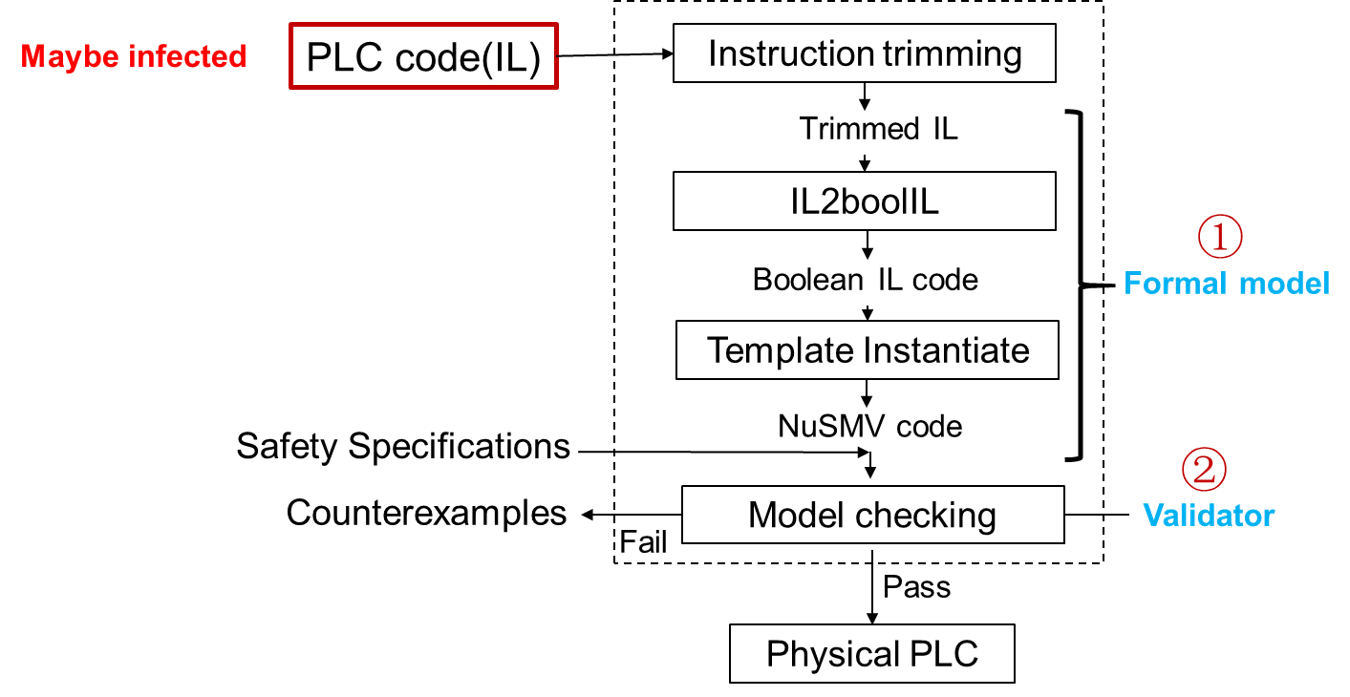
\includegraphics[scale=0.49]{spec/flowchart_spec.png}
		\caption{基于规范的入侵检测流程图}
		\label{fig21}
	\end{figure}

\section{系统建模和入侵检测设计}
\label{sec:matheq}

\subsection{PLC指令表程序介绍}

指令表程序(Instruction  List,IL)是一种较老的PLC编程语言,它使用类似于计算机的一些助记符记号来表示PLC的操作功能,并根据相应的词法和语法写入每一行程序,以实现工业要求的控制目标和运算处理。

指令表程序具有以下特点:

\begin{itemize}
\item 每条指令包含明确的功能而且变量之间的逻辑关系清晰。 
\item 类似于汇编语言,与其他四种编程语言相比更适合现有的程序验证方法。 
\item 系统执行效率高。
\item 和其他四种编程语言可以直接对应。
\end{itemize}

因此,为了真正了解PLC程序变量之间的逻辑关系,实现PLC程序的形式验证,首先我们必须掌握指令表程序,这也是指令表程序成为我们研究对象的重要原因。虽然国际电工委员会在IEC61131-3中定义了国际标准的指令表程序,但为了提高系统效率的实际应用,以西门子,洛克威尔和三菱PLC为代表的厂商都发展自己的具体指令表程序规范。尽管每个公司对于指令表程序具有不同的命名约定,但是这些指令表程序在逻辑级上的含义是相同的。由于我们更多关注指令表语义的逻辑,PLC厂商这个因素不会影响我们的检测研究。本文将以西门子的指令程序语句表(Statement  List,STL)为对象开始相关研究工作。

在西门子S7-200指令系统中,可以分为基本指令和应用指令。 所谓的基本指令,最初是指代替传统继电器控制系统所要求的指令。 随着PLC的功能越来越强大,越来越多的指令被涉及,基本指令的内容也在逐步地扩展。 它包括基本逻辑指令,操作指令,数据处理指令,表函数指令和转换指令。 基本逻辑指令包括基本位操作指令,逻辑堆栈指令,定时器指令,计数器指令和比较指令。 基本逻辑指令构成指令集的基本逻辑运算功能,是所有其他指令应用的基础。 因此,本文选择基本逻辑指令中的公共指令,开始对象的研究工作。表\ref{spec:il}展示了我们涉及到的常用的基本指令。

\newcommand{\tabincell}[2]{\begin{tabular}{@{}#1@{}}#2\end{tabular}}
\begin{table}[!htp]
\centering
\caption{IL指令表基本指令表}
\label{spec:il}
\begin{tabular}{|p{2cm}<{\centering}|p{6cm}<{\centering}|p{6cm}<{\centering}|}
\hline
指令 & 指令类别 & 指令描述 \\
\hline
\end{tabular}
\begin{tabular}{|p{2cm}|p{4cm}|p{6cm}|}
\hline
LD & 逻辑指令 & 装载指令,用于网络块逻辑运算的开始。 \\
\hline
LDN & 逻辑指令 & 装载反指令,用于网络块逻辑运算的开始。 \\
\hline
A & 逻辑指令 & 与指令,用于单个常开触点的串联连接。 \\
\hline
AN & 逻辑指令 & 与反指令,用于单个常闭触点的串联连接。 \\
\hline
O & 逻辑指令 & 或指令,用于单个常开触点的并联连接。 \\
\hline
ON & 逻辑指令 & 或反指令,用于单个常闭触点的并联连接。 \\
\hline
S/R & 逻辑指令 & 置位和复位指令。 \\
\hline
OLD & 逻辑堆栈指令 & 或块指令,用于串联电路块的并联连接。 \\
\hline
ALD & 逻辑堆栈指令 & 与块指令,用于并联电路块的串联连接。 \\
\hline
LPS & 逻辑堆栈指令 & 逻辑入栈指令,也称为分支电路开始指令。从堆栈角度看,LPS指令的作用是把栈顶值复制后压入堆栈。\\
\hline
LRD & 逻辑堆栈指令 & 逻辑读栈指令,从堆栈角度看,LRD将第二个堆栈值复制到堆栈顶部。堆栈没有被弹出,但堆栈顶部的旧数值会被破坏。
 \\
\hline
LPP & 逻辑堆栈指令 & 逻辑出栈指令,也称为分支电路结束指令。从堆栈角度看,LPP将
将堆栈的一个数值弹出堆栈,第二个堆栈数值称为堆栈数值的新顶部。\\
\hline
TON & 逻辑定时器指令 & 接通延时定时器,用于单一时间间隔的定时。 \\
\hline
CTU & 逻辑计数器指令 & 增计数器,首次扫描其值为0,在计数脉冲输入端CU的每个上升沿计数器计数一次直到32767后停止计数,复位输入端有效值为0。 \\
\hline
JMP/LBL & 控制指令 & 跳转指令和标号指令,使主机可根据不同条件进行判断,选择不同的程序段执行程序 \\
\hline

\end{tabular}
\end{table}

\subsection{PLC程序的形式化建模}

\textbf{定义1:} IL程序网络(network)是由3元组迁移函数表示: \[ \mathcal{T_{IL}}=(C,c_0,\leftarrow) \] 其中
\begin{itemize}
  \item $C$ 是IL程序配置集
  \item $ c_0 $ 是IL程序初始配置集
  \item $ \leftarrow $ 是迁移关系
\end{itemize}
这里每一个IL程序配置$c\in C$可以由\[ c=(\sigma,e,E) \] 其中
\begin{itemize}
	\item $\sigma$ 是IL程序变量状态
	\item $ e $ 是IL程序网络中将要执行的变量
	\item $ E $ 是IL程序网络中未执行的变量集
\end{itemize}

因为没有标准的步骤来验证PLC程序,我们形式建模的目的是为了通过生成中间语言来更好地或直接转换为NuSMV输入程序。PLC程序的形式模型分为两个阶段。对于第一步,我们采用指令表(IL)作为我们的主要研究PLC语言程序,并且我们需要在算法1中将IL代码转换为布尔逻辑代码(boolIL),即给出映射算法$\={h}: IL \leftarrow boolIL$使得对于IL程序中的每个将要执行的元素$e$都能映射到boolIL中的表示$a=\={h}(e)$。在网络中执行IL运算符的顺序由下一个映射决定:$2^{IL}\leftarrow IL$根据已经执行的元素集确定接下来执行哪个元素。而在boolIL中这一动作已由程序计数器执行并定义映射$p: boolIL\leftarrow IN$将程序中每一条指令$a$映射到它所在的行数$pc$。相应的我们给出boolIL语言的定义:

\textbf{定义2:} boolIL程序网络(network)是也由3元组迁移函数表示: \[ \mathcal{T_{boolIL}}=(B,b_0,\leftarrow) \] 其中
\begin{itemize}
	\item $B$ 是boolIL程序配置集
	\item $ b_0 $ 是boolIL程序初始配置集
	\item $ \leftarrow $ 是迁移关系
\end{itemize}
这里每一个IL程序配置$b\in B$可以由\[ b=(\sigma,a,pc) \] 其中
\begin{itemize}
	\item $\sigma$ 是boolIL程序变量状态
	\item $ a $ 是boolIL程序网络中将要执行的语句
	\item $ pc $ 是boolIL程序网络中$a$语句所在的程序行号
\end{itemize}

第一步的主要目的是获得二进制函数输出从复杂的IL代码通过逐行解释上下文和语义在程序中。算法1首先将完整的程序划分为多个程序块,然后将每个程序块划分为多个网络块部分并初始化所有的集合。其次,我们对每个逻辑和控制指令执行符号解释以获得二进制函数结果。最后,当实现所有IL程序时,每个结果将从存储器输出。

\begin{algorithm}[!htb]
		\caption{IL2boolIL算法}
		\begin{algorithmic}[1]
			\REQUIRE %算法的输入参数:Input  
			IL程序;
			
			\ENSURE %算法的输出:Output  
			boolIL程序;  
		
			\STATE 将完整程序划分成多个程序块$V'$并将每个程序块划分为多个网络块$F$
			\STATE 初始化并设置$V'= 1,F=\emptyset$;
			\FOR{each $j \in SUM_{所有网络块部分}$}
			\SWITCH{第$j$个网络块部分}
			\CASE {$OP$部分}
			\FOR{each $i \in SUM_{本网络块的总行数}$}
			\SWITCH{第$i$行程序指令}
			\CASE {$LD$($LND$)}
			\STATE 设置相应的变量值为初始值(取反)输入并存入内存; 
			\STATE break;
			\ENDCASE:
			\CASE {$A$($AN$)}
			\STATE 设置相应的变量值为(取反)输入与($\&$)上前一指令的运算结果并存入内存;
			\STATE break;
			\ENDCASE
			\CASE {$O$($ON$)}
			\STATE 设置相应的变量值为(取反)输入或($|$)上前一指令的运算结果并存入内存; 
			\STATE break;
			\ENDCASE
			\CASE {$TON/CTU/S/R$}
			\STATE 定时器/计数器/置位/复位指令,需要进行抽象建模处理; 
			\STATE break;
			\ENDCASE
			\ENDSWITCH
			\ENDFOR
			\ENDCASE
		
			\CASE {$ALD$($OLD$)}
			\STATE 使前两个指令运算结果执行与$\&$(或$|$)操作并将执行结果入栈; 
			\STATE break;
			\ENDCASE
			\CASE {$LPS/LPD/LPP$}
			\STATE 存入/读取/弹出堆栈中前一指令的运算结果;
			\STATE break;
			\ENDCASE
			\CASE {$JMP/LBL$}
			\STATE 控制指令,需要进行抽象建模处理;
			\STATE break;
			\ENDCASE
			\CASE {$=$}
			\STATE 输出内存中的最终结果;
			\STATE break;
			\ENDCASE
			\DEFAULT
			\STATE Return $S_{x_{init}}$
			\ENDDEFAULT
			\ENDSWITCH
			\ENDFOR
			\STATE Return $S_{x_{init}}$
		\end{algorithmic}
	\end{algorithm}

对于步骤二,我们需要通过步骤一的二进制输入函数的输出来实例化验证工具程序模板到可执行代码模型。在我们的工作中,我们采用NuSMV作为我们的模型检查器,因为它支持计算树逻辑(CTL)和线性时间逻辑(LTL)中表达的规范的分析,我们可以从我们的控制系统的安全规范中轻松获得。详细的实例化进度如图\ref{fig2}所示。图\ref{fig2}首先实例化所有输入,输出和pc计数。考虑初始化输入和输出是自动生成过程,因此主要任务是在执行下一个输出语句时为每个case语句分配每个pc执行语句。

\section{实验仿真}
\label{sec:insertimage}

\section{本章小结}
\label{sec:insertimage}

